%----------------------------------------------------------------------------------------
%    PACKAGES AND THEMES
%----------------------------------------------------------------------------------------

\documentclass[aspectratio=169,xcolor=dvipsnames]{beamer}
\usetheme{SimplePlus}

\usepackage{tikz}
\usepackage{hyperref}
\usepackage{graphicx} % Allows including images
\usepackage{booktabs} % Allows the use of \toprule, \midrule and \bottomrule in tables
\usepackage{wrapfig}
\usepackage{listings}
\usepackage[font=small,labelfont=bf]{caption}

%----------------------------------------------------------------------------------------
%    TITLE PAGE
%----------------------------------------------------------------------------------------

\title{Error Based Regression}
\subtitle{HI 743}

\author{Ryan Gallagher}

\institute
{
    Department of Health Informatics and Administration \\
    Zilber College of Public Health \\
    University of Wisconsin - Milwaukee% Your institution for the title page
}
\date{February 20, 2025} % Date, can be changed to a custom date


%----------------------------------------------------------------------------------------
%    PRESENTATION SLIDES
%----------------------------------------------------------------------------------------

\begin{document}
\begin{frame}
    % Print the title page as the first slide
    \titlepage
\end{frame}

%----------------------------------------------------------------------------------------
%    Outline
%----------------------------------------------------------------------------------------

\begin{frame}{Overview}
    % Throughout your presentation, if you choose to use \section{} and \subsection{} commands, these will automatically be printed on this slide as an overview of your presentation
    \tableofcontents
\end{frame}

%----------------------------------------------------------------------------------------
%    Slides
%----------------------------------------------------------------------------------------
\section{Simple Linear Regression}
\subsection{Simple Linear Model}
\begin{frame}{Introduction to Simple Linear Regression}

Simple Linear Regression is a method used to model the relationship between a \textbf{single predictor} variable $X$ and a \textbf{quantitative response variable} $Y$. \\
\bigskip
\textbf{Simple Linear Model:}
{\Large \begin{equation}\label{eq:test}
 Y \approx \beta_0 + \beta_1X
\end{equation}}
Where the \textit{coefficients}
\begin{itemize}
	\item $\beta_0$ is the intercept (value of $Y$ when $X=0$).
	\item $\beta_1$ is the slope (change in $Y$ for a one-unit increase in $X$)
\end{itemize}
\vspace{0.5cm}
We assume that there is approximately a linear relationship between $X$ and $Y$. This is an approximation because there exists some error in our prediction.
\end{frame}
%----------------------------------------------------------------------------------------
\begin{frame}{Simple Linear Regression}
\textbf{Example} -  $X$ may represent TV Advertising and $Y$ may represent Sales. We can regress Sales onto Ads by fitting the model:\\
{\Large $$ \texttt{sales} \approx \beta_0 + \beta_1 \times \texttt{Ads} $$} \\
\vspace{0.5cm}
Interpretation: \textit{For every one-unit increase in \texttt{Ads}, we get a $\beta_1$ unit increase in \texttt{sales}, plus some $\beta_0$.}

\end{frame}
%----------------------------------------------------------------------------------------
\begin{frame}{Simple Linear Regression}
We, however, don't know the true values of $\beta_0$ and $\beta_1$. Thus, we must estimate these coefficients. \\
\bigskip
\textbf{The Prediction Model}:
{\Large\begin{equation}
\hat{y} = \hat{\beta_0} + \hat{\beta_1}x
\end{equation}}
\bigskip

Where $\hat{y}$ indicates a prediction of $Y$ on the basis of $X = x$. \\ 
\bigskip
\textbf{Note}: In machine learning, we use training data to estimate the coefficients, then test how well the model estimates $Y$ in the test data.

\end{frame}
%----------------------------------------------------------------------------------------
\subsection{Statistical Notation}
\begin{frame}{Statistical Notation}
Notation in our Data:
    \begin{itemize}
        \item \textbf{\( x_i \)} – The \( i \)-th observed value of the \textbf{predictor variable} (independent variable).
        \item \textbf{\( y_i \)} – The \( i \)-th observed value of the \textbf{response variable} (dependent variable).
        $$ (x_1, y_1), (x_2, y_2), ..., (x_n, y_n)$$
    \end{itemize}
    Notation in the \textit{True} model:
    \begin{itemize}
        \item \textbf{\( \beta_0 \)} – The \textbf{intercept}, representing the predicted value of \( Y \) when \( X = 0 \).
        \item \textbf{\( \beta_1 \)} – The \textbf{slope}, representing the change in \( Y \) for a one-unit increase in \( X \).
    \end{itemize}
\end{frame}

%----------------------------------------------------------------------------------------

\begin{frame}{Statistical Notation}
Notation in our \textit{Estimated} model:
    \begin{itemize}
        \item \textbf{\( \hat{\beta}_1 \)} – The \textbf{estimated slope} obtained from the data using least squares.
        \item \textbf{\( \hat{\beta}_0 \)} – The \textbf{estimated intercept} obtained from the data.
        \item \textbf{\( \hat{y}_i \)} – The \textbf{predicted value} of \( y_i \), given by:
        \begin{equation}
            \hat{y}_i = \hat{\beta}_0 + \hat{\beta}_1 x_i
        \end{equation}
        \item \textbf{\( e_i \)} – The \textbf{residual} (error) for observation \( i \), calculated as:
        \begin{equation}
            e_i = y_i - \hat{y}_i
        \end{equation}
    \end{itemize}
\end{frame}
%----------------------------------------------------------------------------------------
\subsection{Estimating Coefficients}
\begin{frame}{Estimating the Regression Coefficients}
    We estimate the coefficients \( \beta_0 \) and \( \beta_1 \) using the \textbf{least squares} method.
    
    \bigskip
    
    \textbf{Residual Sum of Squares (RSS):}
    {\large\begin{align}
        RSS &= \sum_{i=1}^{n} (y_i - (\beta_0 + \beta_1 x_i))^2 \\
        &= \sum_{i=1}^{n} e_i^2
    \end{align}}
    
    \bigskip
    
    The \textbf{Least Squares} approach chooses $\hat{\beta_0}$ \& $\hat{\beta_1}$ that minimizes the RSS.
\end{frame}

% Slide 2: Least Squares Estimates and Interpretation
\begin{frame}{Estimating the Regression Coefficients}
\centering
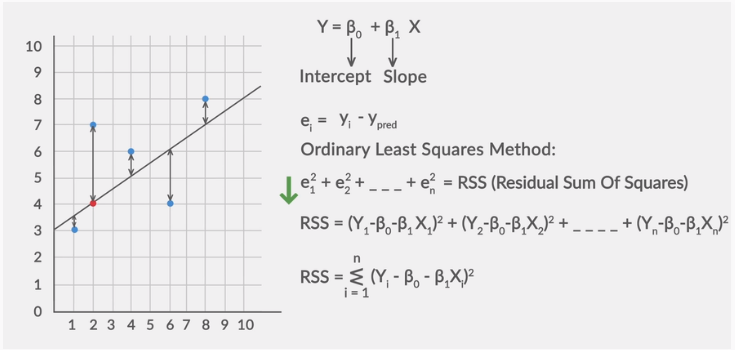
\includegraphics[scale=0.5]{images/RSS.png}

\end{frame}
%----------------------------------------------------------------------------------------
\subsection{Assessing Model Accuracy}
\begin{frame}{Assessing the Accuracy of the Coefficient Estimates}

Our estimates have inherent uncertainty due to sample variability. \\
\bigskip
    \textbf{The Population Regression Model:} \\
    (The best linear approximation of the true relationship between $X$ and $Y$.)
    {\Large\begin{equation}
        Y = \beta_0 + \beta_1 X + \epsilon
    \end{equation}} \\
    Where \( \epsilon \) is a random error term with mean zero. This is a catch-all term for what we miss with this simple model - that the relationship is \textit{probably} not linear.

    \bigskip
    \textbf{The best linear model minimizes $\epsilon$}
    
\end{frame}

%----------------------------------------------------------------------------------------
\begin{frame}{Residual Standard Error (RSE)}
\textbf{RSE} measures how much the actual \( Y \) values deviate from the regression line. It is similar to the standard deviation but applied to regression errors (residuals).
    
    \bigskip
    
    \textbf{Residual Standard Error (RSE):}
    \begin{equation}
        RSE = \sqrt{\frac{1}{n-2} \sum (y_i - \hat{y}_i)^2}
    \end{equation}


    \bigskip

    \textbf{Interpretation:}
    \begin{itemize}
        \item A smaller \( RSE \) means the model fits the data well.
        \item If RSE = 3, on average, the predicted values ($\hat{y}$) differ from actual values ($y$) by about 3 units.
    \end{itemize}
\end{frame}
%----------------------------------------------------------------------------------------
\begin{frame}{\( R^2 \) (R-Squared): Goodness of Fit}
\textbf{\( R^2 \)} measures how well the model explains variation in \( Y \). \( R^2 \) is the proportion of variation in \( Y \) that is explained by \( X \).
    
    \bigskip
    
    \textbf{\( R^2 \) (R-Squared):}
    \begin{equation}
        R^2 = 1 - \frac{RSS}{TSS}
    \end{equation}
    where:
    \begin{itemize}
        \item \( RSS \) = Residual Sum of Squares \( \sum (y_i - \hat{y}_i)^2 \) (unexplained variation).
        \item \( TSS \) = Total Sum of Squares \( \sum (y_i - \bar{y})^2 \) (total variation in \( Y \)).
    \end{itemize}

    \bigskip

    \textbf{Interpretation:}
    \begin{itemize}
        \item \( R^2 \) ranges from 0 to 1.
        \item \( R^2 = 0.8 \) → 80\% of variation in \( Y \) is explained by \( X \).
        \item Higher \( R^2 \) means a better model, but beware of overfitting!
    \end{itemize}
\end{frame}

%----------------------------------------------------------------------------------------

\section{Multiple Linear Regression}
\subsection{Multiple Regression Model}
\begin{frame}{Introduction to Multiple Linear Regression}
\textbf{Multiple Linear Regression} extends simple linear regression to multiple predictors. It helps us understand how multiple variables impact the response variable.


    \bigskip

    \textbf{Multiple Linear Regression Model:}
    \begin{equation}
        Y = \beta_0 + \beta_1 X_1 + \beta_2 X_2 + \dots + \beta_p X_p + \epsilon
    \end{equation}
    where:
    \begin{itemize}
        \item \( Y \) is the response variable.
        \item \( X_1, X_2, ..., X_p \) are predictor variables.
        \item \( \beta_0, \beta_1, ..., \beta_p \) are unknown coefficients.
        \item \( \epsilon \) is the error term.
    \end{itemize}

    \bigskip

    \textbf{Example: Predicting Sales}
    \begin{equation}
        \text{Sales} = \beta_0 + \beta_1 \times \text{TV} + \beta_2 \times \text{Radio} + \beta_3 \times \text{Newspaper} + \epsilon
    \end{equation}
\end{frame}

%----------------------------------------------------------------------------------------
\subsection{Regression Coefficients}
\begin{frame}{Estimating the Regression Coefficients}
    \textbf{Similar to Simple Linear Regression...}
    \begin{itemize}
        \item Use Least Squares to estimate \( \beta_0, \beta_1, ..., \beta_p \).
        \item Choose coefficients that minimize the Residual Sum of Squares (RSS).
    \end{itemize}

    \bigskip
    
    \textbf{RSS Formula:}
    \begin{equation}
        RSS = \sum_{i=1}^{n} (y_i - \hat{y}_i)^2 = \sum_{i=1}^{n} (y_i - (\beta_0 + \sum_{j=1}^{p} \beta_j x_{ij}))^2
    \end{equation}

    \bigskip

    \textbf{How are \( \beta_j \) values found?}
    \begin{itemize}
        \item $\beta_j$ refer to all variables in your model - requires matrix algebra to solve RSS.
        \item R and other statistical tools compute these estimates automatically.
    \end{itemize}
\end{frame}

%----------------------------------------------------------------------------------------
\begin{frame}{Understanding Regression Coefficients}
    \textbf{Interpretation of \( \beta_j \):}
    \begin{itemize}
        \item \( \beta_j \) represents the change in \( Y \) for a one-unit increase in \( X_j \), \textbf{holding all other predictors constant}.
        \item Example: If \( \beta_2 = 0.189 \) is our radio ad coefficient, then a \$1,000 increase in radio advertising increases sales by \textbf{189 units} (given all other coefficients remain constant).
    \end{itemize}

    \bigskip

    \textbf{Caution: Correlation Between Predictors}
    \begin{itemize}
        \item Coefficients can change dramatically if predictors are correlated.
        \item Example: TV and radio spending might be correlated, affecting their individual estimates.
    \end{itemize}
\end{frame}

%----------------------------------------------------------------------------------------

\subsection{Collinearity}
\begin{frame}{Collinearity in Multiple Regression}
    \textbf{Collinearity:}
    \begin{itemize}
        \item When predictor variables are \textbf{highly correlated}, the regression model becomes unstable.
        \item Leads to unreliable coefficient estimates and high standard errors.
    \end{itemize}

    \bigskip

    \textbf{Detecting Collinearity:}
    \begin{itemize}
        \item \textbf{Variance Inflation Factor (VIF)} measures multicollinearity:
        \begin{equation}
            VIF(X_j) = \frac{1}{1 - R^2_{X_j | X_{-j}}}
        \end{equation}
        \item \( VIF > 5 \) suggests collinearity issues.
    \end{itemize}

    \bigskip

    \textbf{Managing Collinearity}
    \begin{itemize}
        \item Remove or combine correlated predictors.
        \item Use other regression techniques (PCA, Ridge Regression)
    \end{itemize}
\end{frame}

%----------------------------------------------------------------------------------------
\subsection{Assessing Model Fit}

\begin{frame}{Model Fit: Adjusted \( R^2 \)}
\textbf{Adjusted \( R^2 \)} improves on \( R^2 \) by considering the number of predictors. Unlike \( R^2 \), it penalizes unnecessary predictors to prevent overfitting.

    \bigskip

    \textbf{Adjusted \( R^2 \):}
    \begin{equation}
        R^2_{\text{adj}} = 1 - \left( \frac{\text{RSS} / (n - p - 1)}{\text{TSS} / (n - 1)} \right)
    \end{equation}

    \bigskip

    \textbf{Interpretation:}
    \begin{itemize}
        \item Higher Adjusted \( R^2 \) → better fit while controlling for complexity.
        \item Adding unnecessary predictors \textbf{decreases} Adjusted \( R^2 \).
        \item Useful for comparing models with \textbf{different numbers of predictors}.
    \end{itemize}
\end{frame}

%----------------------------------------------------------------------------------------

\begin{frame}{Model Fit: Mean Squared Error (MSE)}
\textbf{MSE} measures the average squared difference between actual and predicted values. Lower MSE means the model has \textbf{better predictive accuracy}. This is a standard metric when comparing \textit{most} ML models.

    \bigskip

    \textbf{Formula:}
    \begin{equation}
        MSE = \frac{1}{n} \sum_{i=1}^{n} (y_i - \hat{y}_i)^2
    \end{equation}

    \bigskip

    \textbf{Interpretation:}
    \begin{itemize}
    	\item \textbf{Smaller MSE} → Model predictions are closer to true values.
        \item It quantifies how well the model predicts unseen data.
    \end{itemize}
\end{frame}

%----------------------------------------------------------------------------------------

\subsection{Feature Selection}
\begin{frame}{Feature Selection in Regression}
    \textbf{Why Feature Selection?}
    \begin{itemize}
        \item Not all predictors contribute significantly to the model.
        \item Removing irrelevant features improves interpretability and reduces overfitting.
        \item Can enhance prediction accuracy and model efficiency.
    \end{itemize}

    \bigskip

    \textbf{Types of Features:}
    \begin{itemize}
        \item \textbf{Predictive Features} – Directly useful for estimating \( Y \).
        \item \textbf{Interacting Features} – Not useful alone but important with others.
        \item \textbf{Redundant Features} – Strongly correlated with another predictor.
        \item \textbf{Irrelevant Features} – No useful information for predicting \( Y \).
    \end{itemize}

    \bigskip

    \textbf{Goal:} Select a minimal subset that maintains model performance.
\end{frame}

%----------------------------------------------------------------------------------------

\begin{frame}{Feature Selection Methods}
    \textbf{1. Filter Methods (Pre-Processing)}
    \begin{itemize}
        \item Rank features using statistical metrics (e.g., correlation, mutual information).
        \item Remove low-ranking features before modeling.
    \end{itemize}

    \bigskip

    \textbf{2. Wrapper Methods (Model-Based)}
    \begin{itemize}
        \item Iteratively select the best subset of features by training models.
        \item Common approaches:
        \begin{itemize}
            \item \textbf{Forward Selection} – Start with none, add features stepwise.
            \item \textbf{Backward Selection} – Start with all, remove stepwise.
            \item \textbf{Stepwise Selection} – Combines forward and backward approaches.
        \end{itemize}
    \end{itemize}

    \bigskip

    \textbf{3. Regularization (Shrinkage)}
    \begin{itemize}
        \item Penalizes large coefficients to reduce complexity.
        \item \textbf{LASSO (L1)} forces some coefficients to zero (feature selection).
        \item \textbf{Ridge Regression (L2)} shrinks all coefficients but keeps them nonzero.
    \end{itemize}
\end{frame}


\end{document}